\documentclass[a4paper,14pt, openany, twoside, draft]{extbook} % computer modern font calls
% При завершении (верстке) заменить draft на final!!!!
\usepackage[final]{graphicx}
\graphicspath{{./img/}} % Местонахождение картинок
\usepackage[usenames]{xcolor}
\usepackage{siunitx}
\usepackage{supertabular}
% \usepackage[final]{minted} % Удобный пакет для представления программного кода, требует внешнюю программу и специальные параметры запуска. В отличие от пакета listings поддерживаются русские буквы и utf-8.
%\usemintedstyle{emacs} % Разные стили цвета текста
%\usemintedstyle{tango}
%\usemintedstyle{trac} % better (more bold faces}
%\usemintedstyle{manni} % pastel colors
%\usemintedstyle{bw}    % Черно-белый стиль, следует использовать при верстке печатных документов

%\setminted{breaklines=true,fontsize=\small,funcnamehighlighting=true,python3=true} % Настройка параметров пакета minted

%\newminted{prolog}
%\protect\newminted[proexp]{prolog}{style=bw} % Создание специального окружения для кода языка Prolog.  Окружение позволяет не расцвечивать примеры-запросы.

% Main style definition
% ---------------------
% ISU standard handbook.
%\usepackage[times,fancybot,firamono]{subook} % looks less good than inconsolata
\usepackage[times,fancybot,inconsolata,cambriamath]{subook} % Собственно загрузка стиля.
%\usepackage[fancybot,inconsolata,cambriamath]{subook} % Собственно загрузка стиля.
%\usepackage[times]{subook}

% Заменить в коде кой-что на математические формулы
% http://www.tug.org/texlive/Contents/live/texmf-dist/doc/latex/base/alltt.pdf

% Требования к оформлению Типографии ИГУ
% http://lawinstitut.ru/ru/about/services/izdatelstvo/trebovaniya.html
%

% ISU standard monograph (less restrictive and more artistic)
% Из этого примера можно взять настройки стиля для нашего стиля ;-).
% mag не надо использовать! Он тут чисто исторически остался.
% \usepackage[monograph,mag,times,smalltitles,fancybot,listbib,ptfonts,microtyping]{subook}

% Some artistism for monograph
% ----------------------------
%\makeatletter{}
%\renewcommand\su@chapter@font{\sffamily\sfcpshape\bfseries}
%\renewcommand\su@chapter@font@size{\LARGE}
%\makeatother{}
%\floatname{algorithm}{Процедура}
%\renewcommand{\listalgorithmname}{Список процедур}
%\renewcommand\cftsecnumwidth{5ex}
%\tolerance=5000
%\renewcommand{\chaptername}{Глава}
%\usepackage[final]{hyperref}

\newcommand{\AAA}{\textup{\AA}}
\newcommand{\vect}[1]{\mathbf{#1}}

\definecolor{mygreen}{rgb}{0,0.6,0} % Цвета для отображения комментариев.
\definecolor{mygray}{rgb}{0.5,0.5,0.5}
\definecolor{mymauve}{rgb}{0.58,0,0.82}


\usepackage{tikz}  % Очень мощный пакет для рисования, но и одновременно очень сложный.
\usetikzlibrary{arrows,arrows.meta,shapes} % Библиотеки для пакета.
\usetikzlibrary{shadows}
\newcommand*\keystroke[1]{% Команда используется для отображения нажатий клавиш.
  \tikz[baseline=(key.base)]
    \node[%
      draw,
      fill=white,
      drop shadow={shadow xshift=0.25ex,shadow yshift=-0.25ex,fill=black,opacity=0.75},
      rectangle,
      rounded corners=4pt,
      inner sep=1pt,
      line width=0.7pt,
      font=\footnotesize\sffamily
    ](key) {~#1~\strut}%
  ;%
}

\long\def\rem#1{} % Используется для комментирования больших кусков текста.
\def\emphbib#1{#1} % Заглушка для оформления стилей заголовков книг в списке литературы
%\newenvironment{questions}{\subsubsection*{Вопросы для самопроверки}\begin{enumerate}\itemsep0pt minus 0.3pt\parskip0pt plus 0.3pt}{\end{enumerate}}

%\newtheorem{example}{Пример}[chapter]
\hypersetup{
    bookmarks=true,         % show bookmarks bar?
    unicode=true,           % non-Latin characters in Acrobat’s bookmarks
    pdftoolbar=true,        % show Acrobat’s toolbar?
    pdfmenubar=true,        % show Acrobat’s menu?
    pdffitwindow=false,     % window fit to page when opened
    pdfstartview={FitH},    % fits the width of the page to the window
    pdftitle={Название работы},    % title
    pdfauthor={Автор},     % author
    pdfsubject={О чем идет речь в работе},   % subject of the document
    pdfcreator={EMACS-24.5:AuCTeX},   % creator of the document
    pdfproducer={LuaLaTeX}, % producer of the document
    pdfkeywords={Ключевое слово 1} {Ключевое слово 2} {Ключевое слово 3}, % list of keywords
    pdfnewwindow=true,      % links in new window
    colorlinks=true,       % false: boxed links; true: colored links
    linkcolor=[rgb]{0 0.4 0.1},          % color of internal links (black)
    citecolor=blue,        % color of links to bibliography
    filecolor=black,      % color of file links
    urlcolor=[rgb]{0.3 0.0 0.3}           % color of external links
}

%\renewcommand{\headrulewidth}{1pt}

\clubpenalty=3000
\widowpenalty=3000
%\brokenpenalty=10000
%\floatingpenalty=10000

%% \setdefaultlanguage{russian}
%% \setmainlanguage{russian}
%% \setotherlanguage{english}

%\newenvironment{mygroup}{}{}

\renewcommand\baselinestretch{1.5} % Для диплома.

\definecolor{rclr}{rgb}{0.5,0.1,0.1}
\definecolor{eclr}{rgb}{0,0.5,0.5}
\colorlet{acolor}{blue}
\colorlet{rcolor}{red}
\definecolor{ncolor}{rgb}{0.5,0.5,0.1}
\newcommand{\aaa}[2][acolor]{\noindent\textcolor{eclr}% Использую для пометки места, где надо текста добавить
{+\ [}\textcolor{#1}{#2}\textcolor{eclr}{]}}
\newcommand{\rrr}[2][rcolor]{\noindent% Использую для пометки места, где текста надо убрать
\textcolor{eclr}{-\ [}\textcolor{#1}{#2}\textcolor{eclr}{]}}
\newcommand{\nnn}[2][ncolor]{\noindent% Использую для пометки места, где надо на что-то обратить внимание
\textcolor{eclr}{!\ [}\textcolor{#1}{#2}\textcolor{eclr}{]}}
%\newcommand{\goforth}[1]{$\,\hookrightarrow$\pageref{#1}} % Фича для рисования знака быстрого перехода через раздел, если нет его смысла читать.

% \begin{figure} % Шаблон для включения .pdf_latex - файлов, генерируемых редактором Inkscape
%   \centering
%   \def\svgwidth{\columnwidth}
%   \includesvg{image}
% \end{figure}

%Настройка ниже поджимает абзацы друг к другу, но визуально никак не заметно (пока).
\parskip=0pt plus 0.3pt
\begin{document}
% \itemsep3pt plus 0pt minus 3pt
% \widowpenalty=10000
% \clubpenalty=10000
% \renewcommand\sutitlefontface{\Large\ptsans\nwshape\bfseries}
% \theorembodyfont{\rmfamily}

%\renewcommand{\chaptername}{} % for ISU Handbooks
\renewcommand{\refname}{Список использованных источников} % ... also
\renewcommand{\bibname}{\refname}
\begin{titlepage}
\thispagestyle{empty}
%\aaa{Эта и следующая страница вставляется из .docx}
\begin{center}{\small{}
Министерство образования и науки
Российской Федерации\\
Федеральное государственное бюджетное образовательное\\
учреждение высшего профессионального образования\\
<<Иркутский государственный университет>> \\
Институт математики, экономики и информатики
%\\[2ex]
%    Учреждение Российской академии наук \\
%<<Институт динамики систем и теории управления \\
%Сибирского отделения РАН>>
}
\vfill
\hbox to \linewidth{\hfill\bfseries А.~Л.~Финкельштейн, Т.~Ю.~Черкашина\hfill}
 \vspace{2em}
{\large\bfseries Учебное пособие для физиков}\\
\vspace{1em}
{Учебное пособие для физиков}
\vfill
%\vfill
\vfill
 \textbf{Иркутск 2015}
\end{center}
\end{titlepage}

\clearpage
%\setcounter{page}{2}
\tableofcontents
\clearpage

\chapter*{Введение}
\label{cha:intro}

\section*{Историческая справка}
\label{sec:history}


[http://nuclphys.sinp.msu.ru/introduction/nobelprice.htm ]

[http://www.physchem.chimfak.rsu.ru/Source/History/Persones/Roentgen.html ]

РЁНТГЕН Вильгельм Конрад, (Wilhelm Conrad Röntgen)

\begin{figure}
\centering
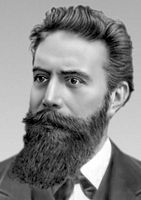
\includegraphics[width=4.794cm,height=6.798cm]{a11-img001.jpg}
\end{figure}
27 марта 1845 г. – 10 февраля 1923 г. Первая Нобелевская премия по физике, 1901 г.

Немецкий физик Вильгельм Конрад Рёнтген родился в Леннепе, небольшом городке в Пруссии, и был единственным ребенком в семье торговца Фридриха Конрада Рёнтгена и Шарлотты Констанцы (в девичестве Фровейн) Рёнтген.

Рёнтген поступил в Утрехтскую техническую школу в 1862 г., но был исключен за то, что отказался назвать своего товарища, нарисовавшего непочтительную карикатуру на нелюбимого преподавателя.

1865 г. был зачислен студентом в Федеральный технологический институт в Цюрихе. Рёнтген работал в физических лабораториях университетов Вюрцбурга, Страсбурга, Гисена и снова Вюрцбурга, до 1872 г. под руководством физика-экспериментатора А.Кундта, потом самостоятельно.

8 ноября 1895 г. профессор университета баварского города Вюрцбурга на юге Германии Вильгельм Конрад Рентген впервые наблюдал неизвестные ранее лучи, проникающие через непрозрачные преграды.

27 ноября того же года шведский изобретатель и промышленник Альфред Бернхард Нобель (1833–1896) подписал в Париже завещание. Этим судьбоносным событиям довелось встретиться через пять лет.

Английский физик Уильям Крукс обнаружил, что стенки стеклянной трубки (трубка Крукса) из которой был откачан воздух с помощью усовершенствованного вакуумного насоса, и в которой вызывали высоковольтный разряд между электродами, флуоресцируют зеленоватым светом. Крукс показал, что лучи испускает отрицательный электрод (помещенный внутрь трубки крестообразный предмет отбрасывал тень на противоположную стенку) и что лучи состоят из некоторой субстанции и несут отрицательный электрический заряд (ударяясь о лопасти легкого колесика, лучи приводили его во вращение, а пучок лучей отклонялся магнитом в сторону, соответствующую отрицательному заряду). В 1878~г. Крукс высказал гипотезу о том, что флуоресценцию вызывают лучи, когда ударяются о стеклянные стенки. Так как отрицательный электрод называется катодом, испускаемое стенками излучение получило название катодных лучей.

Рёнтген повторил некоторые из более ранних экспериментов, в частности показав что исходящие катодные лучи (тогда еще неизвестные) вызывают флуоресценцию экрана, покрытого цианоплатинитом бария. Однажды (это случилось 8 ноября 1895~г.) Рёнтген, чтобы облегчить наблюдения, затемнил комнату и обернул трубку Крукса плотной непрозрачной черной бумагой. К своему удивлению, он увидел на стоявшем неподалеку экране, покрытом цианоплатинитом бария, полосу флуоресценции. Тщательнейшим образом проанализировав и устранив возможные причины ошибок, он установил, что флуоресценция появлялась всякий раз, когда он включал трубку, что источником излучения является именно трубка, а не какая-нибудь другая часть цепи и что экран флуоресцировал даже на расстоянии почти двух метров от трубки, что намного превосходило возможности короткодействующих катодных лучей.

Следующие семь недель он провел, исследуя явление, которое он назвал икс-лучами (т.е. неизвестными лучами). Тень, которую отбрасывал на флуоресцирующий экран проводник от индукционной катушки, создававшей необходимое для разряда высокое напряжение, навела Рёнтгена на мысль об исследовании проникающей способности икс-лучей в различных материалах. Рёнтген заметил, что свинец непроницаем для икс-лучей, и тут сделал поразительное открытие: кости его руки отбрасывали на экран более темную тень, окруженную более светлой тенью от мягких тканей.

Вскоре он обнаружил, что икс-лучи вызывают не только свечение экрана, покрытого цианоплатинитом бария, но и потемнение фотопластинок (после проявления) в тех местах, где икс-лучи попадают на фотоэмульсию. Так Рёнтген стал первым в мире радиологом. В честь него икс-лучи стали называть рентгеновскими лучами.

\begin{figure}
\centering
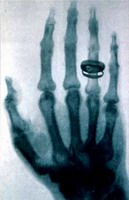
\includegraphics[width=5.546cm,height=8.599cm]{a11-img002.jpg}
\end{figure}
Широкую известность приобрела выполненная Рёнтгеном в рентгеновских лучах фотография (рентгенограмма) кисти руки. На ней, отчетливо видны кости (более плотная костная ткань задерживает икс-лучи, не давая им попасть на фотопластинку) на фоне изображения мягких тканей (задерживающих икс-лучи в меньшей степени) и полоски от колец на пальцах.

После открытия Рёнтгена немецкий физик Макс фон Лауэ высказал блестящее предположение о том, что волновой характер рентгеновского излучения можно было бы доказать, используя в качестве дифракционной решетки регулярно расположенные атомы в кристалле. В 1913 г. эксперимент, предложенный фон Лауэ, был поставлен Вальтером Фридрихом и Паулем Книппингом. Так, открыв неизвестное ранее излучение, Рёнтген внес существенный вклад в ту революцию в физике, которая происходила в начале XX в.

Значение открытия Рентгена подтверждается присуждением еще нескольких нобелевских премий за работы в области рентгеновских лучей:

– в 1914 г., за открытие дифракции рентгеновских лучей (Мах фон Лауэ);  – в 1915 г., за изучение структуры кристаллов с помощью рентгеновских лучей (отцу и сыну Брэггам); Уильям Генри Брэгг и Уильям Лоренс Брэгг. – в 1917 г., за открытие характеристического рентгеновского излучения (Чарльз Баркла);  – в 1924~г., за исследования спектров в диапазоне рентгеновских лучей (Карл Зигбан); – в 1927 г., за открытие эффекта рассеяния рентгеновских лучей на свободных электронах вещества. (Артур Комптон);  – в 1936 г., за вклад в изучение молекулярных структур с помощью дифракции рентгеновских лучей и электронов (Петер Дебай);  – в 1979 г., за разработку метода осевой (рентгеновской) томографии (А.Кормак и Г.Хаунсфилд).

Наиболее заметные открытия, связанные с применением X-лучей

{}- в 1922 г. Нобелевская премия за разработку теории периодической системы элементов, используя закономерности изменения рентгеновских спектров (Нильсу Бору);

{}- 1922 г. Открытие элемента Гафний по рентгеновским спектрам (А.Довийе);

{}- 1925 г. Открытие элемента Рений по рентгеновским спектрам (супруги Ноддак);

{}- 1946 г. Нобелевская премия по физиологии и медицине Герману Меллеру за обнаружение и изучение мутаций под действием рентгеновских лучей;

{}- 1962 г. Нобелевская премия по химии за установление структуры глобулярных белков методом рентгеноструктурного анализа (Джон К. Кендрю~и Макс Ф. Перуц);~

{}- 1964 г. Нобелевским лауреатом по химии стала женщина - англичанка Дороти Кроуфут-Ходжкин: методом рентгено-структурного анализа она определила строение белков и ряда биологически активных соединений;

{}- в 1981 г. Кай Сигбан (сын Карла Сигбана) удостоился Нобелевской премии по физике за разработку рентгеновской электронной спектроскопии - метода широко применяемого в химических исследованиях.

{}- 1988 г. Нобелевская премия по химии за установление трёхмерной структуры фотосинтетического реакционного центра~(Иоганн Дайзенхофер, Хартмут Михель и~Роберт Хубер);

{}- в 2002 г. Нобелевская премия по физике за вклад в астрофизику, который привел к открытию рентгеновских космических источников (Р. Джаккони).

В России уже в январе 1896 г. А.С.Попов в Кронштадте получил рентгеновские снимки для публичных демонстраций. В письме В.Рентгену профессор И.И.Боргман 3 (15) февраля 1896 г. сообщал результаты экспериментов с Х-лучами, выполненных им совместно с А.Л.Гершуном. В приложении к книге с переводом сообщения об открытии Х-лучей был приведен снимок рентгенограммы и утверждалось, что «отпечаток при помощи лучей Рентгена был получен в Физической лаборатории Петербургского университета 12 января, первый снимок руки сделан был 16 января». Вклад в исследование рентгеновских лучей в России в первые годы после открытия Рентгена внесли также другие русские исследователи: П.Н.Лебедев, Б.Б.Голицын, О.Д.Хвольсон, Ю.В.Вульф, А.Ф.Иоффе и др. Н.Г.Егоров организовал первую в России рентгеновскую лабораторию, а А.С.Попов – первый рентгеновский кабинет в Кронштадтском госпитале. В 1897 г. газеты писали, что студент Военно-медицинской академии Н.В.Вихрев сконструировал прибор, с помощью которого можно было делать одновременно два рентгеновских снимка с двух разных точек. Совмещая оба снимка, исследователь получал объемное изображение.

Под руководством А.С.Попова рентгеновскими аппаратами были оборудованы крупные корабли российского флота. Так, на крейсере «Аврора» во время Цусимского сражения были рентгенологически обследованы около 40 раненых матросов, что избавило их от мучительных поисков осколков с помощью зонда.

Применение

Дефектоскопия.

Рентгеноспектральный анализ (по первичным спектрам, в том числе микрозондовый, по флуоресцентным спектрам, в том числе рентгенорадиометрия,

по спектрам поглощения), рентгеноструктурный анализ, рентгеновская микроскопия,

рентгеновская сепарация и др.).

Медицина

медицинская томография

\section{Рентгеновское излучение. Область энергии излучения. Непрерывный и дискретный спектр излучения}
\label{sec:spectrumtype}

Рентгеновские лучи представляют собой электромагнитное излучение в области энергии приблизительно от 0.1 до 150-300 кэВ или в области длин волн приблизительно от 10{}-2 до 102 Å (1 Å (ангстрем) = 10{}-8 см = 0.1 нм).

На рисунке ниже отмечена область рентгеновского излучения (X{}-rays) в шкале электромагнитных волн. [ https:////ru.wikipedia.org/wiki/Файл:EM\_spectrum.svg ]

 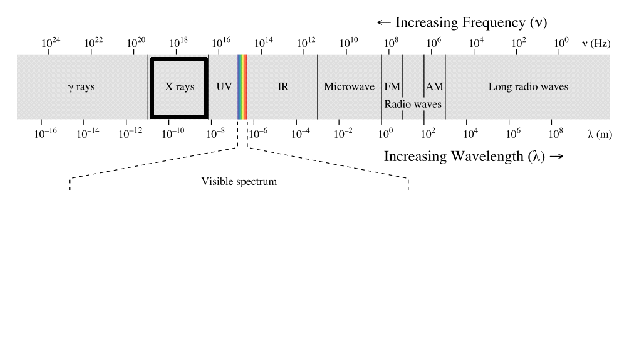
\includegraphics[width=16.595cm,height=7.114cm]{a12-img001.png}

Энергия электромагнитного излучения Ev  связана с длиной волны ${\lambda}$  и частотой электромагнитной волны ${\nu}$  соотношением

 $E_{\nu }=\mathit{h\nu }=\frac{\text{hc}}{\lambda }$, \ \ \ \ \ \ \ \ \ \ \ \ \ \ \ \ (1.1)

где h – постоянная Планка, c – скорость света.

 $E({\text{\textcyrillic{кэВ}}})=\frac{12.398}{\lambda ({\text{\textcyrillic{ангстрем}}})}$\ \ \ \ \ \ \ \ \ \ \ \ \ \ (1.2)

Два главных процесса обуславливают возникновение рентгеновского излучения.

Рентгеновское излучение образуется в результате ионизации внутренних электронных оболочек атомов заряженными частицами или фотонами и в результате торможения (потери энергии) электронов или других заряженных частиц в поле атомного ядра и атомных электронов.

Характеристическое излучение возникает вследствие электронных переходов между дискретными уровнями атома. В результате удаления электрона с внутренней оболочки атома вакансия заполняется электронами другой оболочки. Возникает излучение, энергия которого равна разности энергий уровней атома. На рисунке ниже приведена схема вероятных переходов между уровнями атома. Два конкурирующих процесса наблюдаются при возникновении вакансии на внутренней оболочке – флуоресценция и оже-эффект. Эффект Оже более вероятен для низких атомных номеров, в то время как рентгеновское флуоресцентное излучение более вероятно для высоких атомных номеров.

\begin{flushleft}
\tablefirsthead{}
\tablehead{}
\tabletail{}
\tablelasttail{}
\begin{supertabular}{|m{6.866cm}|m{8.0130005cm}|}
\hline
{\selectlanguage{russian} [Warning: Draw object ignored]} &
{\selectlanguage{russian} [Warning: Draw object ignored]}\\\hline
{\selectlanguage{russian} Флуоресценция. После взаимодействия фотона достаточной энергии с атомом и возникновения вакансии в K{}-оболочке она заполняется электроном с L{}-оболочки. Атом покидает рентгеновский фотон характеристической K${\alpha}${}-линии и фотоэлектрон.} &
{\selectlanguage{russian} Эффект Оже. После возникновения вакансии в K{}-оболочке она заполняется электроном с L{}-оболочки. Возникает фотон, энергия которого достаточна для ионизации уровня в M{}-оболочке. Атом покидает Оже-электрон.}\\\hline
\end{supertabular}
\end{flushleft}
Каждый элемент имеет характеристические K, L и М-серии. Легкие элементы имеют только K- линии, элементы среднего  диапазона атомных номеров могут испускать и K и L - спектры, в то время как тяжелые элементы имеют K, L и М-спектры.  На рисунке приведена диаграмма основных рентгеновских переходов K, L и М-серии и фрагмент спектра K{}-серии Sr  на котором видны группы K${\alpha}${}- и K${\beta}${}-линий. Индексами ${\alpha}$, ${\beta}$, ${\gamma}$ обозначаются линии в порядке убывания интенсивности.

\begin{flushleft}
\tablefirsthead{}
\tablehead{}
\tabletail{}
\tablelasttail{}
\begin{supertabular}{|m{8.0130005cm}|m{8.485001cm}|}
\hline
{\selectlanguage{russian} [Warning: Draw object ignored] 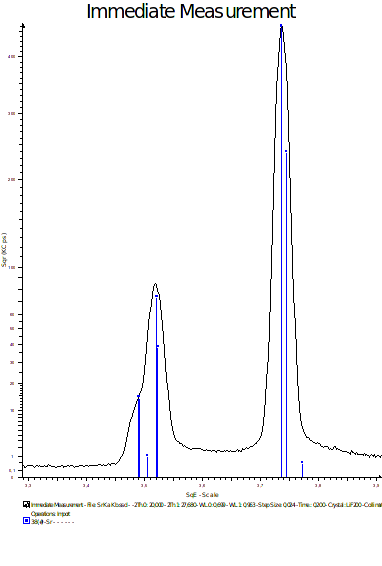
\includegraphics[width=7.44cm,height=11.128cm]{a12-img002.png} } &
{\selectlanguage{russian}  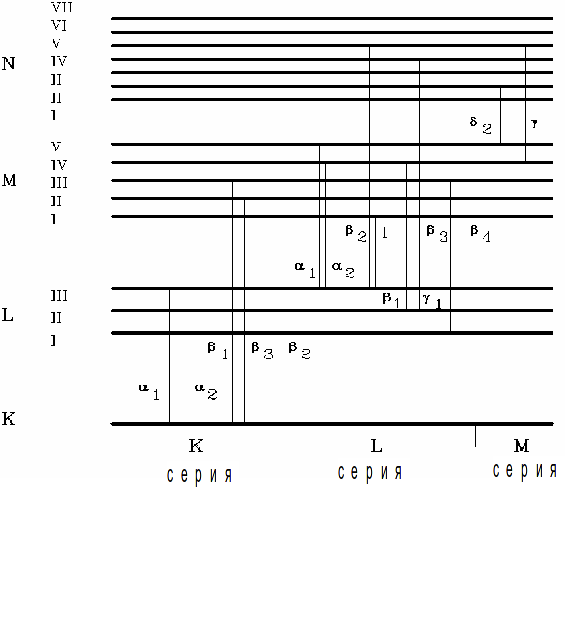
\includegraphics[width=8.285cm,height=9.442cm]{a12-img003.png} }\\\hline
\end{supertabular}
\end{flushleft}
Тормозное рентгеновское излучение образуется в результате торможения электронов (или других заряженных частиц) в поле ядра атомов материала анода, имеет непрерывный спектр в области длин волн больше коротковолновой границы  $\lambda _0$, которая определяется ускоряющим электроны напряжением V. Интенсивность тормозного спектра увеличивается с атомным номером материала анода.

На рисунке интенсивность непрерывного спектра дана при трех различных напряжениях для одного и того же материала анода.

 $\lambda _0(\overset{\circ }{A})=\frac{12.398}{V({\text{\textcyrillic{кВ}}})}$ 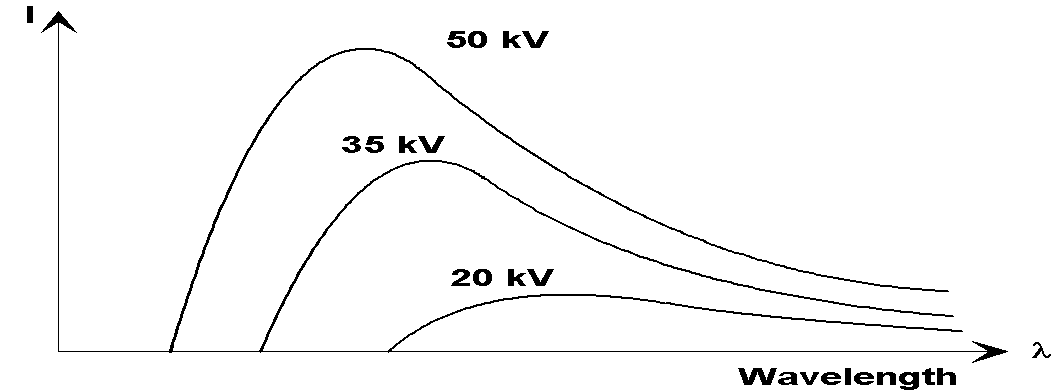
\includegraphics[width=9.049cm,height=5.348cm]{a12-img004.png}

На рисунке ниже в общих чертах изображен спектр рентгеновской трубки с анодом из родия. На фоне непрерывного тормозного спектра присутствуют характеристические линии K{}- и L{}-серии Rh.

 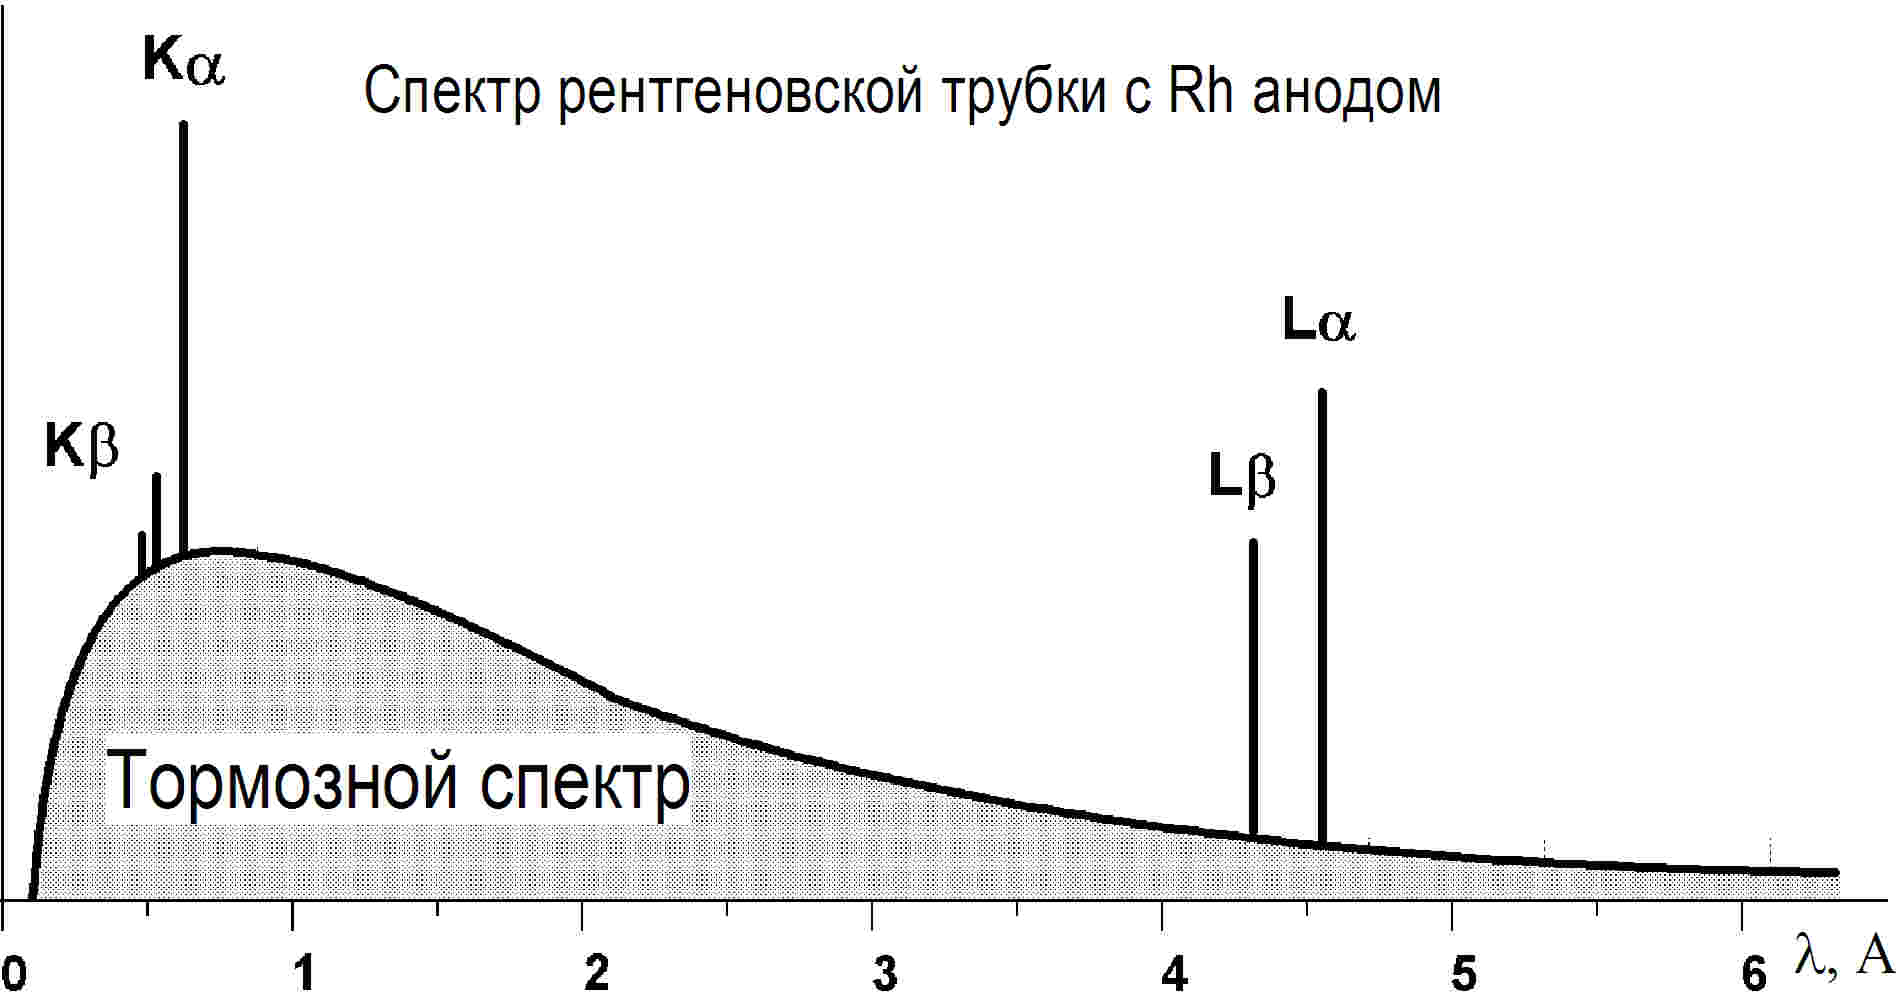
\includegraphics[width=14.944cm,height=7.92cm]{a12-img005.jpg}

2. Модели атома

2.1. Модель атома Бора. Энергии уровней водородоподобного атома.

[ Зоммерфельд А. Строение атома и спектры. Т. 1. М.: ГИТИ. 1956. Гл. 2.  С. 80. ]

В модели атома Бора электроны вращаются вокруг ядра по круговым (или эллиптическим орбитам). Орбита электрона определяется двумя условиями: одно классическое и одно квантовое.

Классическое условие определяет равновесие между центробежной силой и силой кулоновского притяжения

 ${\text{ma}}\omega ^2=\frac{{\text{Ze}}^2}{a^2}$ \ \ или \ \ \ \ \ \ \ \ \ \ \ \

 ${\text{ma}}^3\omega ^2={\text{Ze}}^2$\ \ ,\ \ \ \ \ \ \ \ \ \ \ \ (2.1)

где m – масса электрона, a и ${\omega}$ – радиус орбиты и угловая скорость обращающегося электрона, e – заряд электрона. Ze – заряд ядра атома. Угловая скорость электрона и его скорость  вдоль траектории v определены выражением для центробежной силы

 $\frac{{\text{mv}}^2} a={\text{mv}}\omega ={\text{ma}}\omega ^2$.\ \ \ \ \ \ \ \ \ \ \ \ \ \ (2.2)

Квантовое условие накладывается на момент количества движения вращающегося электрона

 $2\mathit{\pi p}={\text{nh}}$.\ \ \ \ \ \ \ \ \ \ \ \ \ \ \ \ (2.3)

Момент количества движения равен

 $p={\text{mva}}={\text{ma}}^2\omega $ .\ \ \ \ \ \ \ \ \ \ \ \ \ \ (2.4)

И, таким образом, квантовое условие имеет вид

 ${\text{ma}}^2\omega =\frac{{\text{nh}}}{2\pi }$.\ \ \ \ \ \ \ \ \ \ \ \ \ \ \ \ (2.5)

Делением соотношения (2.1) на (2.4) получим:

 $v=\mathit{a\omega }=\frac{2\pi {\text{Ze}}^2}{{\text{nh}}}$,\ \ \ \ \ \ \ \ \ \ \ \ \ \ (2.6)

 $a=\frac{n^2h^2}{4\pi ^2{\text{mZe}}^2}$ , \ \  $\omega =\frac{n^2h^2}{4\pi ^2{\text{mZe}}^2}$.\ \ \ \ \ \ \ \ \ \ (2.7)

В случае атома водорода Z=1 и радиус первой боровской орбиты (n=1) равен

 $a_0=\frac{h^2}{4\pi ^2{\text{me}}^2}$\ \ = 5.29 10{}-9 см ( или 0.529 Å )\ \ \ \ \ \ \ \ \ \ (2.8)

Далее введем величину

 $\alpha =\frac{v_0} c$, где v0 – скорость электрона водородного атома на первой боровской орбите, с – скорость света. Согласно (2.6) имеем

 $\alpha =\frac{v_0} c=\frac{2\mathit{\pi e}^2}{{\text{hc}}}$= 1/137.\ \ \ \ \ \ \ \ \ \ \ \ \ \ (2.9)

Величина ${\alpha}$ -  постоянная тонкой структуры имеет существенное значение при рассмотрении электромагнитного взаимодействия.

Полная энергия равна сумме кинетической и потенциальной энергии W=Eкин+Eпот .

 $E_{{\text{\textcyrillic{кин}}}}=\frac{{\text{mv}}^2} 2=\frac{2\pi ^2{\text{mZ}}^2e^4}{n^2h^2}$,\ \ \ \ \ \ \ \ \ \ \ \ \ \ (2.10)

 $E_{{\text{\textcyrillic{пот}}}}=-\frac{{\text{Ze}}^2} a=-\frac{4\pi ^2{\text{mZ}}^2e^4}{n^2h^2}$\ \ \ \ \ \ \ \ \ \ \ \ \ \ (2.11)

И, таким образом,

 $W_n=-\frac{2\pi ^2{\text{mZ}}^2e^4}{n^2h^2}$\ \ \ \ \ \ \ \ \ \ \ \ (2.12)

В модели Бора также возможны эллиптические орбиты той же энергии. Для каждой энергии имеется n возможных орбит с моментами импульса:

\begin{figure}
\centering
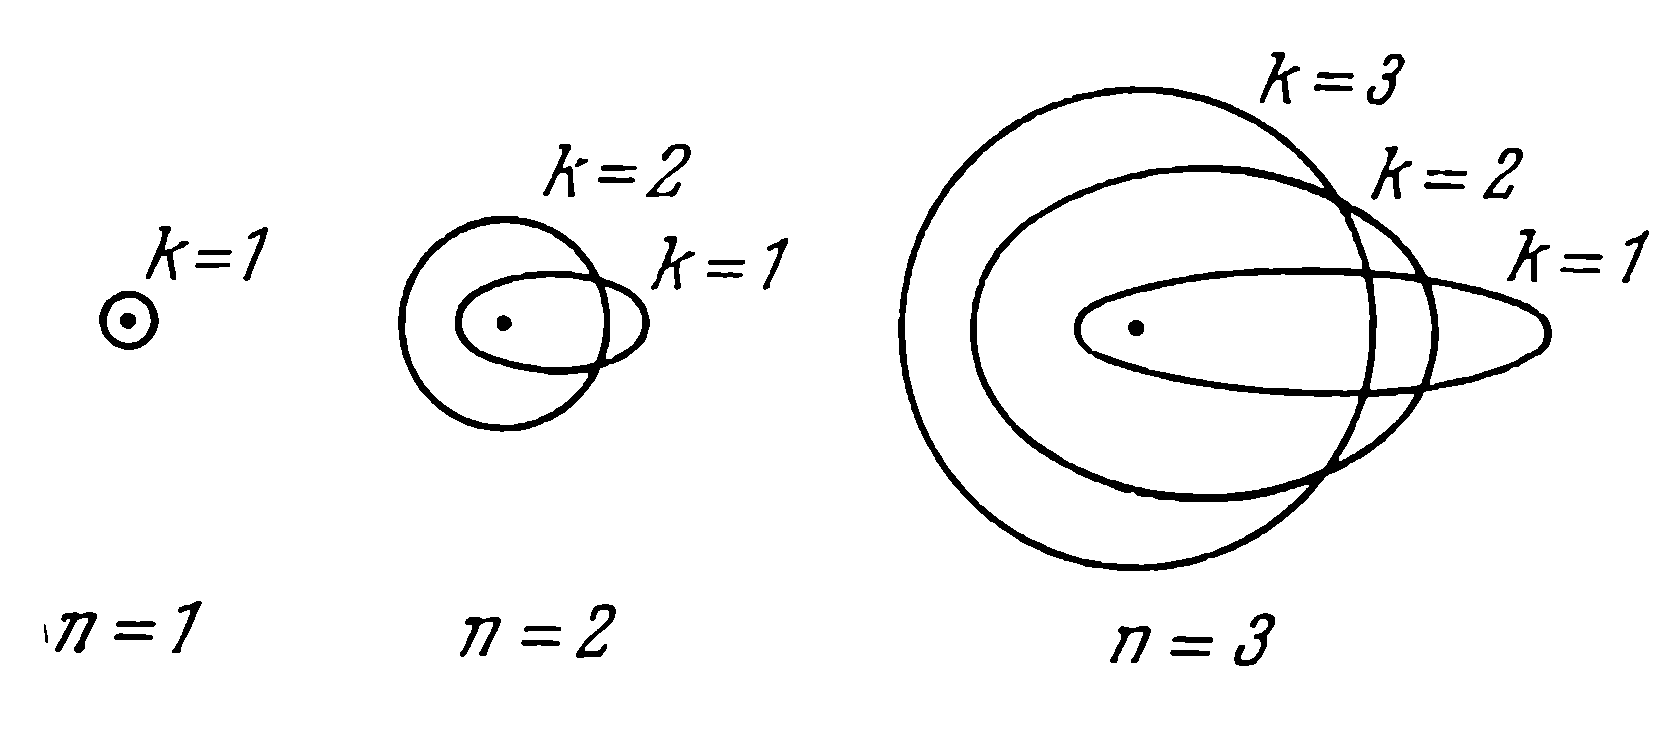
\includegraphics[width=7.091cm,height=3.157cm]{a21-img001.png}
\end{figure}
 $L={\text{kh}}/2\pi $, k = 1, 2, 3, …, n ( $k\le n$).

При k=n орбита является круговой, другие орбиты – эллипсы.

Совокупность орбит с определенным n называют оболочками. Оболочку n=1 называют K{}-оболочкой, оболочку n=2 L{}-оболочкой, и т.д. M{}-, N{}-, O{}-оболочки.

Энергия излучения  $E_{\gamma }$ будет равна разности энергий уровней (оболочек), между которыми происходит переход электрона

 $E_{\gamma }={\text{hv}}=W_n-W_m$,\ \ \ \ \ \ \ \ \ \ \ \ (2.13)

 $E_{\gamma }={\text{RhcZ}}^2(\frac 1{n^2}-\frac 1{m^2})$,\ \  $v={\text{RZ}}^2(\frac 1{n^2}-\frac 1{m^2})$,\ \ \ \ \ \ \ \ (2.14)

где введена постоянная Ридберга  $R=\frac{2\pi ^2{\text{me}}^4}{{\text{ch}}^3}$.

Выражение (11) с хорошей точностью позволяет оценить энергии некоторых линий характеристического рентгеновского излучения, например, K${\alpha}${}-линий. Следует только учесть, что на K{}-оболочке (n=1) в соответствии с принципом Паули находится два электрона и электрон, находящийся на L{}-оболочке (n=2) находится в поле ядра, экранированного оставшимся на K{}-оболочке электроном. Т.е. для перехода L${\rightarrow}$K вместо Ze следует взять эффективное значение (Z{}-1)e. Тогда

 $E_{\gamma }=13.6{\text{\textcyrillic{эВ}}}\cdot (Z-1)^2(\frac 1{n^2}-\frac 1{m^2})$,\ \ \ \ \ \ \ \ \ \ \ \ (2.15)

где постоянная величина в формуле (2.14)  Rhc=13.6 выражена в единицах эВ.

Из выражения (2.15) для излучения K${\alpha}$1{}-линии Na находим E${\gamma}$=1020 эВ. Точное измеренное значение энергии излучения NaK${\alpha}$1{}-линии равно 1040.98 эВ.

Для излучения L{}-серии, когда электрон переходит с M{}-оболочки (n=3) на L{}-оболочку (n=2), он чувствует ядро, экранированное оставшимися 9-ю электронами на K{}- и L{}-оболочках. Следует ожидать, что эффективный заряд будет равен (Z{}-9)e. В действительности экранирование будет несколько меньше. Для учета этого эффекта вводят постоянную экранирования ${\sigma}$. Т.е. эффективный заряд будет равен (Z{}-${\sigma}$)e.

Так для излучения L${\alpha}${}-линии молибдена Z=42 и  ${\sigma}{\approx}$7, и

 $E_{\gamma }=13.6{\text{\textcyrillic{эВ}}}\cdot (Z-\sigma )^2(\frac 1{n^2}-\frac 1{m^2})=13.6{\text{\textcyrillic{эВ}}}\cdot (42-7)^2(\frac 1{2^2}-\frac 1{4^2})$ = 2301 эВ.

Измеренное значение энергии излучения MoL${\alpha}${}-линии равно 2292 эВ.

Таким образом, довольно простая полуклассическая теория Бора позволила с удивительной точностью оценивать энергии характеристических линий рентгеновского спектра.

Из выражения (2.14) непосредственно следует эмпирический закон Мозли

 $\sqrt v$\~{} $Z$,\ \ \ \

где v{}- частота электромагнитных волн характеристических линий рентгеновского спектра.

\section{Статистическая модель атома Томаса-Ферми. Электронная плотность.}
\label{sec:statmodel}

[Левич В.Г., Вдовин Ю.А., Мямлин В.А. Курс теоретической физики. Т. 2. М.: Наука. 1971. Гл. 11. С. 285.]

Для тяжелых многоэлектрнных атомов получил применение метод Томаса-Ферми, в котором предполагается, что взаимодействие между электронами является достаточно слабым и электроны атома можно рассматривать как идеальный ферми-газ при абсолютном нуле температуры.

В вырожденном ферми-газе электроны попарно заполняют квантовые состояния, так что на каждую пару приходится ячейка фазового пространства объемом (2${\pi}$\textlatin{[127?]})3 . При этом в пространстве импульсов заполнены все ячейки с импульсом в интервале  $0\le p\le p_{\text{max}}$. Значение pmax можно выразить через плотность электронного газа n (среднее число электронов в единице объема)

 ${\text{dn}}=\frac{8\pi }{(2\pi \hbar )^3}p^2{\text{dp}}$.

Интегрируя от p=0 до р=pmax получим

 $p_{\text{max}}^3=\frac 3{8\pi }(2\pi \hbar )^3n$.

Плотность заряда ${\varrho}$=en

\begin{equation*}
\rho =\frac{8\mathit{\pi e}}{3(2\pi \hbar )^3}p_{\text{max}}^3
\end{equation*}
pmax может быть связан с потенциалом ${\varphi}$(r) с помощью следующего рассуждения. Энергия электрона E, связанного в атоме, всегда не положительна, т.е.

 $E=\frac{p^2}{2m}+\mathit{e\varphi }(r)\le 0$.

Полагаем, что потенциал ${\varphi}$(r) вне атома обращается в нуль, откуда для максимального импульса, при E=0, находим

 $p_{\text{max}}=\sqrt{-2{\text{me}}\varphi (r)}$.

Поэтому плотность электронного заряда связана с потенциалом соотношением

 $\rho =\frac{8\mathit{\pi e}}{3(2\pi \hbar )^3}\left(\sqrt{-2{\text{me}}\varphi (r)}\right)^3$.

Для сферически симметричного потенциала электростатического поля можно записать уравнение Пуассона

 $\Delta \varphi =-4\pi\rho$,

или

 $\frac 1{r^2}\frac{d^2(\mathit{r\varphi })}{{\text{dr}}^2}=\frac{4e}{3\pi \hbar ^3}\left(\sqrt{-2{\text{me}}\varphi (r)}\right)^3$.

Граничные условия для нейтрального атома следующие. Потенциал должен обращаться в нуль на больших расстояниях, т.е.

 $\varphi \rightarrow 0$ при  $r\rightarrow \propto ?$.

Вблизи ядра поле чисто кулоновское

 $\varphi (r)\rightarrow \frac{{\text{Ze}}} r$ при  $r\rightarrow 0$.

Для получения решения переходят к безразмерным величинам –

 $\chi =\frac{\mathit{r\varphi }}{{\text{Ze}}}$,  $x=\frac r d$,

где e – модуль заряда. d – постоянная величина с размерностью длины.

Полагая d равным

 $d=\frac 1 2\left(\frac{9\pi ^2}{16}\right)^{1/3}\frac{\hbar ^2}{{\text{me}}^2}\frac 1{Z^{1/3}}=0.88\frac{a_0}{Z^{1/3}}$, где a0 – радиус первой боровской орбиты,

для ${\chi}$  приходим к уравнению

 $\frac{d^2\chi }{{\text{dx}}^2}=\frac{\chi ^{3/2}}{\sqrt x}$,

при граничных условиях

 $\chi \rightarrow 1$ при  $x\rightarrow 0$,

 $\chi \rightarrow 0$ при  $x\rightarrow \propto ?$.

Границы применимости метода Томаса-Ферми связаны с границами применимости квазиклассического приближения, т. е.  $r\text{{\textgreater}{\textgreater}}a/Z$. На больших расстояниях r\~{}a квазиклассическое приближение снова становится неприемлемым, т.е.  $a/Z\text{{\textless}{\textless}}r\text{{\textless}{\textless}}a$. Следствием модели Томаса-Ферми является оценка размера нейтрального атома. В сфере радиусом приблизительно равным  $R=1.33{\text{aZ}}^{1/3}$ заключена половина полного электронного заряда.

Плотность электронов в атоме связана с потенциалом и функцией  $\chi $

 $\rho (r)=\frac{8\mathit{\pi e}}{3(2\pi \hbar )^3}\left(\sqrt{-2{\text{me}}\varphi (r)}\right)^3$= $\left(32Z^2/9\pi \right)^2\left[\frac{\chi (x)} x\right]^{3/2}$.

Плотность электронов определяет амплитуду рассеяния рентгеновских лучей на атомах

 $f=F^2(q)$,  $\hbar q=2\lambda ^{-1}\text{sin}(\vartheta /2)$, где ${\lambda}$,  $\vartheta $ - длина волны излучения и угол рассеяния.

 $F(q)=4\pi \int \rho (r)\frac{\text{sin}({\text{qr}})}{{\text{qr}}}r^2{\text{dr}}$.\ \ \ \

2.3. Уравнение Шредингера для атома водорода.

 [P. Кристи и  А. Питти. Строение вещества: введение в современную физику. «Наука». 1969. С. 392. ]

Атом водорода состоит из электрона и протона. Так как масса протона в 1836 раз больше массы электрона, можно пренебречь движением ядра и рассматривать электрон, движущийся в кулоновском поле ядра. Потенциальная энергия в кулоновском поле ядра равна  $V(r)=-\frac{{\text{Ze}}^2} r$ , где Ze – заряд ядра (для водорода, конечно, Z=1).

Стационарное уравнение Шредингера для электрона, движущегося в поле ядра, имеет вид

 $\left[-\frac{\hbar ^2}{2m}\nabla ^2+V(r)\right]\psi (r)=\mathit{E\psi }(r)$.\ \ \ \ \ \ \ \ \ \ \ \ (2.16)

Или в сферических координатах

 $-\frac{\hbar ^2}{2m}\frac 1{r^2}\frac{\partial }{\partial r}r^2\frac{\partial \psi }{\partial r}+\frac 1{2{\text{mr}}^2}L^2\psi -\frac{{\text{Ze}}^2} r\psi =\mathit{E\psi }$,\ \ \ \ \ \ \ \ \ \ (2.17)

где  $L^2=-\hbar ^2\left[\frac 1{\text{sin}\vartheta }\frac{\partial }{\partial \vartheta }\text{sin}\vartheta \frac{\partial }{\partial \vartheta }+\frac 1{\text{sin}^2\vartheta }\frac{\partial ^2}{\partial \varphi ^2}\right]${}- оператор момента импульса. Если волновая функция соответствует состояниям с определенным импульсом, то

 $L^2\psi =l(l+1)\hbar ^2\psi $\ \ \ \ \ \ \ \ \ \ \ \ \ \ (2.18)

Волновая функция может быть представлена в виде произведения функции, зависящей от r и функции, зависящей от угловых переменных

 $\psi (r,\vartheta ,\varphi )=R(r)Y(\vartheta ,\varphi )$.\ \ \ \ \ \ \ \ \ \ \ \ (2.19)

В результате получается уравнение

 $-\frac{\hbar ^2}{2m}\frac 1{r^2}\frac d{{\text{dr}}}r^2\frac{{\text{dR}}}{{\text{dr}}}+\left[\frac{l(l+1)\hbar ^2}{2{\text{mr}}^2}-\frac{{\text{Ze}}^2} r\right]R={\text{ER}}$\ \ \ \ \ \ \ \ (2.20)(1)

Решения уравнения с отрицательной энергией, которые удовлетворяют граничным условиям при  $r=0$ и  $r\rightarrow \propto ?$, будут давать допустимые энергии электрона в водородоподобном атоме.

Рассмотрим волновые функции при l=0.

Определим параметр

\begin{equation*}
\gamma =\sqrt{-\frac{2{\text{mE}}}{\hbar }=\sqrt{\frac{2m|E|}{\hbar }}}
\end{equation*}
Решение уравнения (2.20), удовлетворяющее условию конечности волновой функции при больших r, ищется в виде

 $R_n=\overset{n-1}{\underset{i=0}{\sum }}C_ir^ie^{-\gamma r},\quad n\geq 1$.

Опуская подробности вычислений, отметим, что условие конечности волновой функции накладывает ограничение для параметра

\begin{equation*}
\gamma =\gamma _n=Z/{\text{na}}_0
\end{equation*}
и, следовательно, определяет спектр энергии уровней

 $E=E_n=-\frac{\hbar ^2Z^2}{2{\text{ma}}_0^2n^2}=-\frac{{\text{me}}^4Z^2}{2\hbar ^2n^2}=-13.6\frac{Z^2}{n^2}({\text{\textcyrillic{эВ}}})$.\ \ \ \ \ \ \ \ \ \ (2.21)

Последнее выражение совпадает с выражением для энергии уровней в теории Бора.

Волновая функция основного состояния (n=1) , будет иметь вид

 $R_1=C_0e^{-\frac{{\text{Zr}}}{a_0}}$.

Постоянная  $C_0$ определяется из условия нормировки

 $\overset{\propto }{\underset 0{\int }}4\mathit{\pi r}^2|R|^2{\text{dr}}=1$.

Тогда волновая функция атома водорода в основном состоянии имеет вид

 $R_1=\frac 1{\sqrt{\mathit{\pi a}_0^3}}e^{-\frac r{a_0}}$.\ \ \ \ \ \ \ \ \ \ \ \ \ \ \ \ (2.22)

И электронная плотность

 $\rho (r)=|R|^2=\frac 1{\mathit{\pi a}_0^3}e^{-\frac{2r}{a_0}}$. \ \ \ \ \ \ \ \ \ \ \ \ \ \ (2.23)

На рисунке ниже приведена зависимость электронной плотности, определяемой волновой функцией атома водорода (сплошная линия), и электронная плотность согласно модели Томасу-Ферми. Видно различие на малых и больших расстояниях  $r/a_0$. Плотность по Томасу-Ферми медленно спадает при   $r/a_0${\textgreater}3-4  и эта область, где нарушается условие применимости модели.

 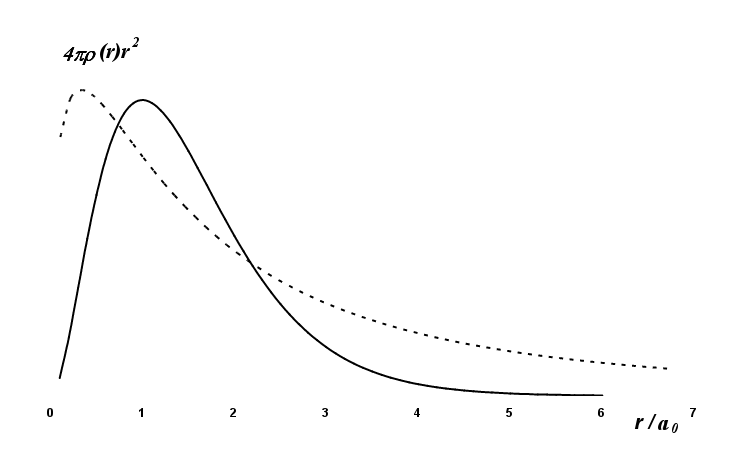
\includegraphics[width=10.421cm,height=6.514cm]{a2324-img001.png}

В общем случае, волновая функция определяется тремя квантовыми числами (n, l, ml ) в соответствии с тремя координатами  $(r,\vartheta ,\varphi )$. ml – магнитное квантовое число, которое определяет собственные значения оператора проекции момента импульса, зависящего от координаты ${\varphi}$, на выделенное направление ось z

 $L_z\psi _m=\frac{\hbar } i\frac{\partial }{\partial \varphi }\psi _m=m_l\hbar \psi _m$.

ml – может принимать значения от –l до l, включая 0, т.е. 2l+1 значений.

Энергетические уровни атома водорода зависят только от главного квантового числа, т.е. волновые функции, имеющие одно и то же n, но различные азимутальные и магнитные квантовые числа, принадлежат одному энергетическому уровню. Такая ситуация называется вырождением.

Уравнение Шредингера не учитывает собственный момент электрона – «спин». Собственный момент электрона – спин, был установлен Гаудстмитом и Уленбеком (1926 г.) при наблюдении расщепления некоторых спектральных линий и впервые обнаружен в опытах Штерна и Герлаха (1921 г.). Возможные значения квантового числа собственного момент электрона ms {}-1/2 и +1/2. Значение спина s=1/2.

Для описания состояния электрона в атоме вводят квантовое число, определяющее полный момент импульса системы

 $j=l\pm s$.

Полный момент импульса системы складывается из орбитального момента и спина электрона.

В результате учета релятивистских поправок выражение для энергии уровней водородоподобного атома может быть записано в следующем виде [Блохин]

 $E_n=-{\text{Rhc}}\frac{M_z}{M_z+m}\left[\frac{Z^2}{n^2}+\alpha ^2\frac{Z^4}{n^4}\left(\frac n{j+1/2}-\frac 3 4\right)\right]$,\ \ \ \ \ \ \ \ \ \ (2.24)

где Mz – масса ядра атома с атомным номером Z. Поскольку ${\alpha}$=1/137 малая величина, второй член в квадратных скобках имеет значение для относительно больших Z.

Точное решение уравнение Шредингера найдено только для атома водорода. Для остальных атомов используют приближенные численные методы решения. Приближенный метод расчета волновых функций электронов в атомах, получивший широкую известность, был предложен Хартри (1927 г.). Метод был назван методом самосогласованного поля и заключается в том, что волновая функция атома представляется в виде суперпозиции волновых функций отдельных электронов, которые движутся в самосогласованном поле, создаваемом ядром и всеми остальными электронами. В этом приближении уравнение Шредингера может быть записано в виде

 $\hat H\psi =\mathit{E\psi }$,   $\hat H=\left[-\frac{\hbar ^2}{2m}\overset N{\underset i{\sum }}\nabla _i^2-\overset N{\underset i{\sum }}\frac{{\text{Ze}}^2}{r_i}+\overset N{\underset i{\sum }}\overset N{\underset{j\neq i}{\sum }}\frac{e^2}{|r_i-r_j|}\right]$.

В методе Хартри волновая функция атома представляется в виде суперпозиции волновых функций отдельных электронов. Слэттер предложил искать радиальные одноэлектронные функции в виде

 $\psi _n=A_nr^{n\ast -1}\text{exp}(-\gamma _n\frac r{a_0})$, где  $n\ast ?${}- эффективное главное квантовое число,  $\gamma _{n,l}=\frac{Z-\sigma _{n,l}}{n\ast a_0}$.

Фок добавил в уравнение слагаемое, связанное с так называемым обменным взаимодействием. Уравнения самосогласованного поля называют уравнениями Хартри-Фока-Слэттера (ХФС, HFS).

\section{Распределение электронов в атомах.}
\label{sec:electron-in-athoms}

[ Блохин М.А. Физика рентгеновских лучей. М.: ГИТТЛ, 1957. С. 17. ]

Значение главного квантового числа n определяет электронную оболочку, к которой относится электрон

n = \ \ 1\ \ 2\ \ 3\ \ 4\ \ 5\ \ 6

оболочка: \ \ K\ \ L\ \ M\ \ N\ \ O\ \ P

Тип состояния определяется значением азимутального квантового числа

l = \ \ 1\ \ 2\ \ 3\ \ 4\ \ 5

тип:\ \ s\ \ p\ \ d\ \ f\ \ g\ \

Для данного квантового числа n  существует 2l+1 значений магнитного квантового числа m и два значения спинового квантового числа ms=${\pm}$1/2. При заданном n число l может принимать значения 0, 1, …., n{}-1. Таким образом полное число различных комбинаций трех квантовых чисел l, m и ms при данном n равно сумме

 $\overset{n-1}{\underset{l=0}{\sum }}2(2l+1)=2n^2$.  ( т.е. 2, 8, 18, 32, …… при n=1, 2, 3, 4,…...).

В соответствии с принципом Паули два электрона не могут иметь один и тот же набор квантовых чисел  n, l, m и ms . Следовательно, в оболочке с главным квантовым числом n может находить не более 2n2 электронов. Распределение электронов по состояниям принято записывать следующим образом

1s2 .

Первая цифра дает значение главного квантового числа, буква обозначает тип состояния и азимутальное квантовое число, верхний индекс обозначает число электронов, находящихся в этом состоянии.

В таблице ниже приведено распределение электронов в атомах благородных газов.

 2 He  1s2

10 Ne  1s2  2s2  2p6

18 Ar  1s2  2s2  2p6  3s2  3p6  3d10

36 Kr  1s2  2s2  2p6  3s2  3p6  3d10  4s2 4p6  4d10

54 Xe  1s2  2s2  2p6  3s2  3p6  3d10  4s2 4p6  4d10  5s2  5p6

Совокупность электронов, занимающих состояния с различными l и   $j=l\pm s$ называют подоболочками или подуровнями.

В таблице ниже приведено распределение электронов для первых трех оболочек по подуровням и их обозначения.

\begin{flushleft}
\tablefirsthead{}
\tablehead{}
\tabletail{}
\tablelasttail{}
\begin{supertabular}{|m{0.7cm}|m{1.9449999cm}|m{0.68cm}|m{1.726cm}|m{2.892cm}|m{1.04cm}|m{1.8499999cm}|m{2.504cm}|}
\hline
\centering{\selectlanguage{english} n} &
{\centering\selectlanguage{russian} Уровень,\par}

\centering{\selectlanguage{russian} оболочка} &
\centering{\selectlanguage{english} l} &
\centering{\selectlanguage{russian} Орбита} &
\centering{\selectlanguage{english} m} &
\centering{\selectlanguage{english} j} &
\centering{\selectlanguage{russian} Под-оболочка} &
{\centering\selectlanguage{russian} Число электронов\par}

{\centering{\selectlanguage{russian} на подуровне}}\\\hline
{\selectlanguage{english} 1} &
{\selectlanguage{english} K} &
{\selectlanguage{english} 0} &
{\selectlanguage{english} s} &
{\selectlanguage{english} 0} &
{\selectlanguage{english} 1/2 } &
{\centering{\selectlanguage{russian} {}-}} &
{\centering{\selectlanguage{russian} 2}}\\\hline
{\selectlanguage{english} 2} &
{\selectlanguage{english} L} &
{\selectlanguage{english} 0}

{\selectlanguage{english} 1} &
{\selectlanguage{english} s}

{\selectlanguage{english} p} &
{\selectlanguage{english} 0}

{\selectlanguage{english} {}-1, 0, +1} &
{\selectlanguage{english} 1/2 }

{\selectlanguage{english} 1/2}

{\selectlanguage{english} 3/2 } &
{\centering\selectlanguage{russian} LI\par}

{\centering\selectlanguage{russian} LII\par}

{\centering{\selectlanguage{russian} LIII}} &
{\centering\selectlanguage{russian} 2\par}

{\centering\selectlanguage{russian} 2\par}

{\centering{\selectlanguage{russian} 4}}\\\hline
{\selectlanguage{english} 3} &
{\selectlanguage{english} M} &
{\selectlanguage{english} 0}

{\selectlanguage{english} 1}

{\selectlanguage{english} 2} &
{\selectlanguage{english} s}

{\selectlanguage{english} p}

{\selectlanguage{english} d} &
{\selectlanguage{english} 0}

{\selectlanguage{english} {}-1, 0, +1}

{\selectlanguage{english} {}-2, -1, 0, +1, +2} &
{\selectlanguage{english} 1/2 }

{\selectlanguage{english} 1/2}

{\selectlanguage{english} 3/2}

{\selectlanguage{english} 3/2}

{\selectlanguage{english} 5/2 } &
{\centering\selectlanguage{russian} MI\par}

{\centering\selectlanguage{russian} MII\par}

{\centering\selectlanguage{russian} MIII\par}

{\centering\selectlanguage{russian} MIV\par}

{\centering{\selectlanguage{russian} MV}} &
{\centering\selectlanguage{russian} 2\par}

{\centering\selectlanguage{russian} 2\par}

{\centering\selectlanguage{russian} 4\par}

{\centering\selectlanguage{russian} 4\par}

{\centering{\selectlanguage{russian} 6}}\\\hline
\end{supertabular}
\end{flushleft}


\chapter{Атом водорода}
Атом водорода образует простейшую атомную систему, состоящую из положительно заряженного ядра, называемого протоном, и обращающегося вокруг него единственного отрицательно заряженного электрона.  Спектр излучения атома водорода может быть понятен на основе представлений о допустимых энергетических уровнях, даваемых формулой
\begin{equation}
  \label{eq:Hydrogen}
E_n=-\frac{13,6}{n^2}\;\text{\emph{эв}},\qquad n=1,2,3,\ldots
\end{equation}
Любая теория электронной структуры материи должна объяснить, почему эти и только эти энергетические уровни являются допустимыми.  Теория Бора не совсем корректна, но из нее наглядно можно получить верные значения энергетических уровней атома водорода при квантовании момента импульса:
\begin{equation}
  \label{eq:2}
L=k\hslash;\qquad k=1,2,3,\ldots
\end{equation}
Уравнение Шредингера предсказывает тот же самый энергетический спектр, что и теория Бора.  Это может быть доказано квантовомеханическим путем.  Решение уравнения Шредингера для электрона, движущегося в стационарном поле кулоновского ядра, описывает не только энергетические уровни электрона и спектр, но и форму атомных орбиталей.  Мы увидим, что квантование момента импульса в волновой механике возникает из требования конечности волновой функции.

\section{Уравнение Шредингера для атома водорода}
\label{sec:shred:H}

Потенциальная энергия электрона в кулоновском поле ядра равна
\begin{equation}
  \label{eq:potenergy}
V(r)=-Ze^2/r,
\end{equation}
где $Ze$~--- заряд ядра.  Рассмотрим общий случай, т.~е. $Z>1$.  Тогда уравнение Шредингера будет иметь вид
\begin{equation}
  \label{eq:shred1}
-\frac{\hslash^2}{2m}\;\frac{1}{r^2}\;\frac{\partial}{\partial r}\;r^2\;\frac{\partial \psi}{\partial r}+\frac{1}{2mr^2}\;{\mathbf{L}}^2\psi-\frac{Ze^2}{r}\;\psi=E\psi.
\end{equation}
Если волновая функция $\psi$ соответствует состоянию с определенным моментом импульса, то согласно уравнению полного момента импульса $L^2=L_{l}^2=l(l+1)\;\hslash^2$ получим
\begin{equation}
  \label{eq:impuls}
{\vect{L}}^2\psi=l(l+1)\hslash^2\psi.
\end{equation}
Если представить функцию $\psi(r, \theta, \phi)$ в форме $\psi (r, \theta, \phi)=R(r)Y(\theta, \phi)$, то множитель $Y(\theta, \phi)$ сокращается.  В результате получается уравнение
\begin{equation}
  \label{eq:shred2}
-\frac{\hslash^2}{2m}\;\frac{1}{r^2}\;\frac{d}{dr}\;r^2\;\frac{dR}{dr}+
\left[\frac{l(l+1)\hslash^2}{2mr^2}-\frac{Ze^2}{r}\right]R=ER.
\end{equation}
Те решения уравнения \ref{eq:shred2} с отрицательной энергией, которые удовлетворяют соответствующим граничным условиям при $r=0$ и $r=\infty$, будут давать допустимые энергии электрона в атоме водорода.
\begin{equation}
  \label{eq:wavefunction}
R_1=C_0e^{-\gamma_1r}=C_0e^{(-{Zr}/{a_0})}.
\end{equation}

\newpage
\chapter*{Фундаментальные постоянные}
{http://physics.nist.gov/cuu/Constants/index.html}

%[Фундаментальные постоянные]{\protect\href{http://physics.nist.gov/cuu/Constants/index.html}{Фундаментальные постоянные}}
%\url{http://physics.nist.gov/cuu/Constants/index.html}

$\mathbfit{c}$  скорость света =  \textbf{2.99}79\,$\cdot$\,10\textsuperscript{8} м/сек % 10${}^8$

$\mathbfit{e}$  заряд электрона = 1.602\,$\cdot$\,10\textsuperscript{-19} кулон

$m_ec^2$  энергия массы покоя электрона = \textbf{5.11}0034\,$\cdot$\,10\textsuperscript{5} эВ = 511 кэВ

$\mathbfit{b}$  барн = 10\textsuperscript{-28} м\textsuperscript{2} = 10\textsuperscript{-24} см\textsuperscript{2}

$r_e=e^2/(m_ec^2)$  классический радиус электрона = \textbf{2.81}79380\,$\cdot$\,10\textsuperscript{-15} м $\approx$ 2.82\,$\cdot$\,10\textsuperscript{-5} $\AAA$

$\mathbfit{r_{e^2}}$ = \textbf{7.94}0775\,$\cdot$\,10\textsuperscript{-30} м\textsuperscript{2}  = \textbf{0.079}40775 $\mathbfit{b}$ (барн)

$\mathbfit{\sigma_r}$ = $8\pi r_e^2/3$ поперечное сечение для классического томсоновского рассеяния от электрона = \textbf{6.65}2448\,$\cdot$\,10\textsuperscript{-29} м\textsuperscript{2} = 0.66552448 $\mathbfit{b}$

$\mathbfit{\alpha}$ = $2\pi e^2/hc$ постоянная тонкой структуры = \textbf{7.29}73506\,$\cdot$\,10\textsuperscript{-3} = 1/137.03604 $\approx$ 1/137

$\mathbfit{a_0}$ = $r_e/\alpha^2$ первый Боровский радиус электрона  = \textbf{5.29}17706\,$\cdot$\,10\textsuperscript{-11} м = 0.52917706 $\AAA$

$\lambda(\AAA)$  длина волны фотона = \textbf{12.39}852/E кэВ

$\mathbfit{\hslash}$ = $h/2\pi$ постоянная Планка = \textbf{4.13}5667\,$\cdot$\,10\textsuperscript{-18} кэВ\,$\cdot$\,с

$\mathbfit{\hslash}$ = \textbf{6.62}607\,$\cdot$\,10\textsuperscript{-34} Дж\,$\cdot$\,с

$\mathbfit{N_A}$  число Авогадро = \textbf{6.022}140857(74)\,$\cdot$\,10\textsuperscript{23} моль\textsuperscript{-1}

$\mathbfit{R_H}$ = $me^4/4\pi c\hslash^3$ постоянная Ридберга для атома водорода = \textbf{109677.58}3407 см\textsuperscript{-1}

1 ферми = 1 фемтометр = 1 фм = 1\,$\cdot$\,10\textsuperscript{-15} м

$\mathbfit{R_p}$ радиус протона = 0.8775(51)\,$\cdot$\,10\textsuperscript{-15} м = 0.8775(51) фм

\clearpage{}
 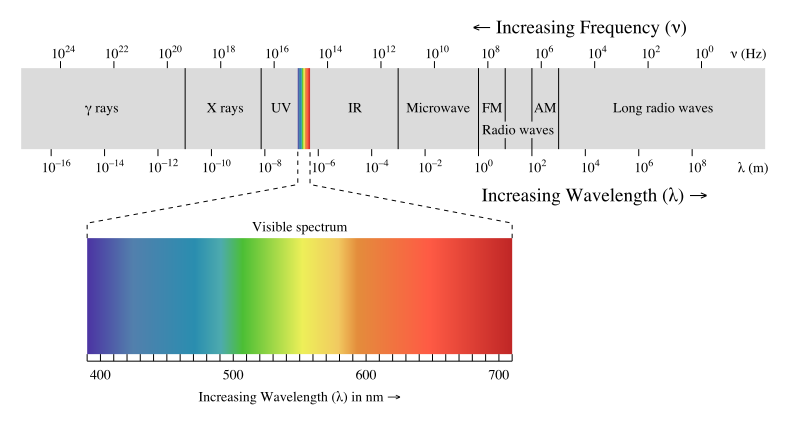
\includegraphics[width=16.866cm,height=9.022cm]{EMRad-img001.png}

https://ru.wikipedia.org/wiki/\%D0\%A4\%D0\%B0\%D0\%B9\%D0\%BB:EM\_spectrum.svg

 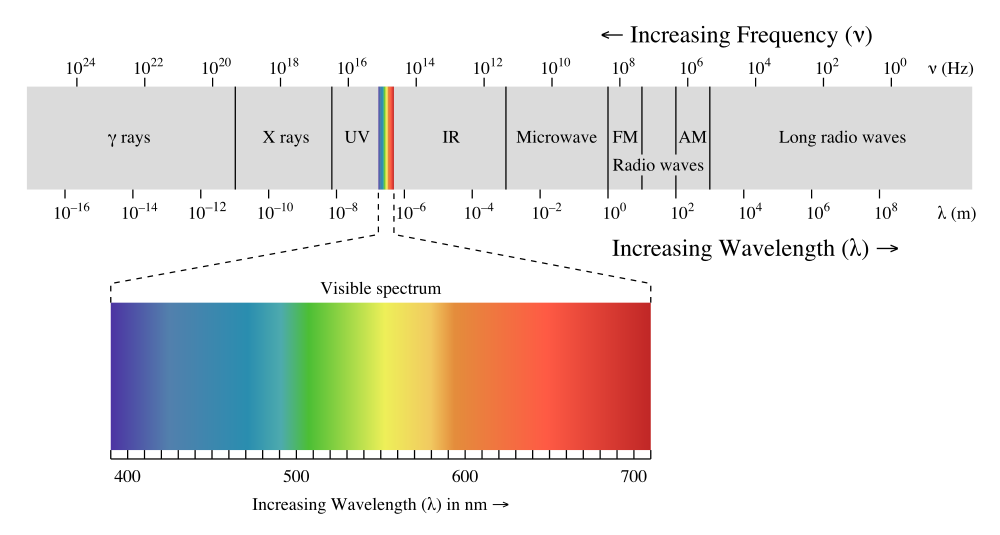
\includegraphics[width=15.665cm,height=8.382cm]{EMRad-img002.png}

 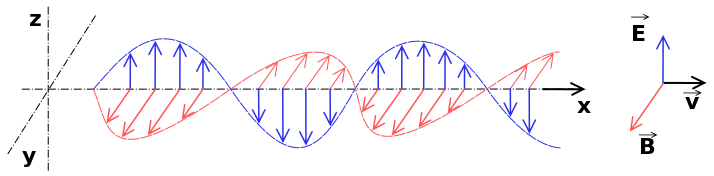
\includegraphics[width=14.713cm,height=3.627cm]{EMRad-img003.png}

http://nuclphys.sinp.msu.ru/introduction/nobelprice.htm




\end{document}

%%%%%%%%%%%%%%%%%%%%%%%%%%%%%%%%%%%%%%%%%%%%%%%%%%%

% Local Variables:
% TeX-parse-self: t
% TeX-auto-save: t
% TeX-master: t
% End:
